\section{Software design}
\label{sec:software}

\pkg{amore} is organised as a single pipeline whose stages each correspond to a
small set of exported functions: \emph{canonicalise} an event log,
\emph{sample} non-events, \emph{compute} endogenous statistics, \emph{fit} a
model, and \emph{check} the fit. The same pipeline runs in two directions --- a
simulation module generates synthetic event streams in the package's own
canonical form, so simulated and observed data flow through the identical
downstream machinery. This section walks through the stages in order, documents
the \code{rem} S3 contract that unifies the three estimation backends, describes
the goodness-of-fit family (which is restricted to the linear case-control fit),
catalogues the nine bundled datasets, and closes with a worked end-to-end
example on \code{classroom\_events}.

\subsection{Preprocessing}
\label{sec:software-preprocess}

\paragraph{Canonicalisation.}
\code{standardize\_event\_log()} maps an arbitrary event table to the package's
\code{amore\_event\_log} contract: three columns \code{sender}, \code{receiver},
\code{time}, with \code{sender}/\code{receiver} coerced to character and
\code{time} to numeric. The source column names are configurable
(\code{sender\_col}, \code{receiver\_col}, \code{time\_col}), and switches
control sorting by time, dropping of incomplete rows (\code{drop\_nas}),
self-loops (\code{drop\_loops}), duplicate \((s,r,t)\) triples
(\code{remove\_duplicates}), and a strict-monotonic-time assertion
(\code{strictly\_increasing\_time}); \code{keep\_extra} preserves any additional
covariate columns. The returned object carries the \code{amore\_event\_log}
class so that downstream functions can recognise a canonicalised log. A
companion \code{attach\_static\_covariates()} joins per-actor attribute tables
onto the stream.

\paragraph{Non-event sampling.}
Fitting a relational event model by the case-control device requires, for each
observed event (the \emph{case}), one or more non-events (the \emph{controls})
drawn from the risk set \citep{lerner2020}. \code{sample\_non\_events()}
implements this with three orthogonal axes. The \code{scope} argument fixes the
candidate pool: \code{"all"} uses every actor observed in the log,
\code{"appearance"} restricts to actors already present by the focal time, and
\code{"citation"} restricts receivers to previously active targets. The
\code{mode} argument selects the design (\code{"one"} matched-set vs.\
\code{"two"} permuted), and \code{risk} governs the risk set itself:
under \code{risk = "remove"} a dyad is dropped from its own control pool once it
has fired (and any dyad firing at the focal timestamp is treated as a concurrent
event, not an eligible non-event), which is the correct convention for
non-repeatable processes such as species invasion. Structurally ineligible
dyads can be excluded wholesale through \code{exclude\_pairs}, a two-column
\((\text{sender}, \text{receiver})\) table. The number of controls per case is
\code{n\_controls}, and \code{seed} makes the draw reproducible.

\paragraph{Endogenous features.}
\code{compute\_endogenous\_features()} computes the requested statistics on the
sampled case-control table. The key semantic subtlety is that controls must read
the \emph{true} network history without themselves polluting it: a sampled
non-event that never occurred should not update degrees, reciprocity, or recency
state for later rows. This is handled by the \code{history\_log} argument. When
the true event log is passed as \code{history\_log}, only rows whose
\((\text{sender}, \text{receiver}, \text{time})\) triple appears in that log
update the running network state, while all other rows (the sampled controls)
have their statistics computed against that state but never enter it. The
default catalogue is \code{c("sender\_outdegree", "receiver\_indegree",
"reciprocity", "recency")}; \code{half\_life} parameterises the exponentially
weighted recency variants. The full catalogue comprises 74 numeric statistics
plus the \code{sender\_receivers\_set} list-column, which returns, per row, the
set of receivers the row's sender has previously reached (joined downstream to an
external lookup to build set-valued covariates). Of the 74 numeric statistics,
66 are computed by a C++ fast path and 8 are pure-R fallbacks; the
\code{cpp\_supported\_stats()} helper reports which statistics the compiled
engine handles. The \code{history\_log} semantics are honoured natively only on
the C++ path; the R fallback raises an error if \code{history\_log} is supplied
for an R-only statistic. A \code{widen\_case\_control()} reshaper converts a long
case-\(k\)-control table to the wide case-1-control layout used by the \code{gam}
backend, emitting \code{<cov>\_ev}, \code{<cov>\_nv}, and \code{d\_<cov>}
(event-minus-control) columns; the 0/1 indicator and stratum columns are
auto-detected (the package's own \code{event} column, or \code{eventnet}'s
\code{IS\_OBSERVED}) when not named explicitly.

\subsection{Simulation}
\label{sec:software-simulation}

The simulation module generates event streams from a specified intensity and
returns them in the same canonical form the fitter consumes, so a simulated log
can be passed directly to \code{sample\_non\_events()} or, with \code{wide =
TRUE}, straight into \code{rem()}. Two engines share a single endogenous-state
machine: an exact Gillespie sampler and an approximate \(\tau\)-leap sampler
that trades exactness for speed and converges to the exact process only as the
leap interval shrinks. Both are pure R. The teaching simulators for
time-varying non-linear and hyper-event models attach the ground-truth
generating functions as an attribute on the returned object, so that recovery
experiments can compare estimates against the truth that produced the data
(Section~\ref{sec:validation}).

\subsection{The \code{rem()} fitter and its S3 contract}
\label{sec:software-rem}

\code{rem()} is the unified front-end. It takes a formula, a preprocessed
case-control \code{data} frame, and a \code{method}, and dispatches to one of
three backends:

\begin{verbatim}
rem(formula, data, method = c("gam", "clogit", "nn"),
    case = NULL, stratum = NULL, time = NULL,
    k = NULL, gam_method = NULL, nn = nn_control(), ...)
\end{verbatim}

The \code{"clogit"} backend fits a conditional logistic regression on a
case-\(k\)-control design via \code{survival::clogit()}, with strata taken from
\code{stratum} or derived as \code{cumsum(case == 1)} for the blocked
case-then-controls layout. The \code{"nn"} backend fits a multilayer perceptron
that scores every candidate in a stratum and is trained on the softmax over each
risk set --- this is the \emph{same} risk-set conditional-logistic partial
likelihood that \code{clogit} maximises, with a learned non-linear intensity in
place of the linear predictor. The \code{"gam"} backend is different in kind: it
fits the algebraically-related \emph{degenerate} case-1-control binomial
logistic regression of \citet{boschi2025rhem}, in which the response is the
constant \(1\) and the linear predictor is built from event-minus-control
differences. It does not form risk-set strata or a softmax; it coincides with a
two-element conditional logit only under a single matched control. The
\code{gam} backend is therefore the route to smooth, time-varying, non-linear,
and random-effect terms, which the formula expresses as \code{tv(x)},
\code{nl(x)}, \code{tvnl(x)}, and \code{re(x)} respectively, delegating to
\code{mgcv}.

All three backends return an object of class \code{"rem"} --- a list holding the
underlying fit (\code{\$fit}), the \code{method}, the \code{formula}, the parsed
\code{terms}, and the observation count \code{n}. The S3 methods delegate to the
inner fit object: \code{print.rem()} reports the method, formula, and \(n\);
\code{summary.rem()}, \code{coef.rem()}, \code{plot.rem()},
\code{logLik.rem()}, and \code{predict.rem()} forward to the backend's
corresponding method. For \code{method = "nn"} there is deliberately no
coefficient table --- \code{coef()} returns \code{NULL}, \code{summary()}
reports in-sample (and, with a validation split, held-out) concordance, and
\code{plot(type = "pdp")} draws per-feature partial-dependence curves. The
neural backend is pure R with no extra dependencies, its analytic gradients
hand-derived and verified against numerical differentiation; it accepts
numeric covariates only and provides no uncertainty quantification.
Architecture and training are configured through \code{nn\_control()}
(hidden-layer sizes, activation, epochs, Adam learning rate, L2 penalty,
validation fraction and early-stopping patience, feature standardisation, and
seed). Besides the joint multilayer perceptron, \code{nn\_control(architecture
= "additive\_spline", spline\_df, batch\_strata)} selects the additive
B-spline architecture of Section~\ref{sec:framework-nn-additive}: per-covariate
basis expansions under a single linear layer, trained on the same partial
likelihood, with optional mini-batching over strata for large event logs. Dependency posture is deliberately light: \code{survival} and
\code{Rcpp} are Imports, while \code{mgcv} is only suggested and the \code{gam}
backend raises an informative error at call time if it is absent.

\subsection{Goodness of fit}
\label{sec:software-gof}

\pkg{amore} ships the cumulative martingale-residual goodness-of-fit family of
\citet{boschi2025gof}. Each entry point builds, through a shared internal routine, a single
case-control sample (drawn at \code{n\_controls = 1}, the paper's NCC \(m=2\)
setup) and a single fitted partial-likelihood model:
\code{gof\_univariate()} tests one covariate via the supremum of the normalised
cumulative score process, whose null distribution is a standard Brownian bridge,
so its p-value follows the Kolmogorov--Smirnov series;
\code{gof\_multivariate()} tests a \(q\)-dimensional smooth or random-effect
term against a \(q\)-dimensional Brownian bridge with an empirical (simulated)
p-value; \code{gof\_global()} forms a Cauchy-combination omnibus statistic with
an analytic p-value; and \code{gof\_auxiliary()} runs a multiplier Monte Carlo
test. A standalone \code{martingale\_residuals()} returns the per-row residuals
for diagnostic plotting.

The single most important scoping fact is that \textbf{this family supports the
linear case-control fit only}. All four entry points route through an internal
fitter that fits a no-intercept binomial GLM on case-minus-control differences
and hard-rejects any effect specification other than \code{"linear"}:

\begin{verbatim}
bad <- model != "linear"
if (any(bad)) {
  stop("Only effect type \"linear\" is supported here. Got: ",
       paste(unique(model[bad]), collapse = ", "))
}
\end{verbatim}

Internally the cumulative residual process is re-centred by subtracting a linear
ramp so that it ends at zero at the maximum-likelihood estimate --- a heuristic
alignment to the score-subtraction step of the Boschi--Wit construction --- and
the number of matched controls is fixed at one. These are the relevant
limitations: the GOF family does not yet cover non-linear or time-varying fits,
nor \(m>2\) nested case-control designs.

\subsection{Bundled datasets}
\label{sec:software-data}

The package ships nine documented data objects spanning roughly two orders of
magnitude in event count (Table~\ref{tab:datasets}): six directed event streams,
two per-actor attribute tables, and one exogenous distance matrix. Each event
stream is built by a script under \code{data-raw/} from a public source with a
recorded DOI, and four of the streams carry the Unix epoch of \code{time = 0} as
\code{attr(., "unix\_origin")} on the data frame, allowing absolute timestamps to
be recovered. Figure~\ref{fig:datasets-rate} shows the event-rate profiles and
Figure~\ref{fig:datasets-degrees} the degree distributions across the streams.

\begin{figure}[t]
\centering
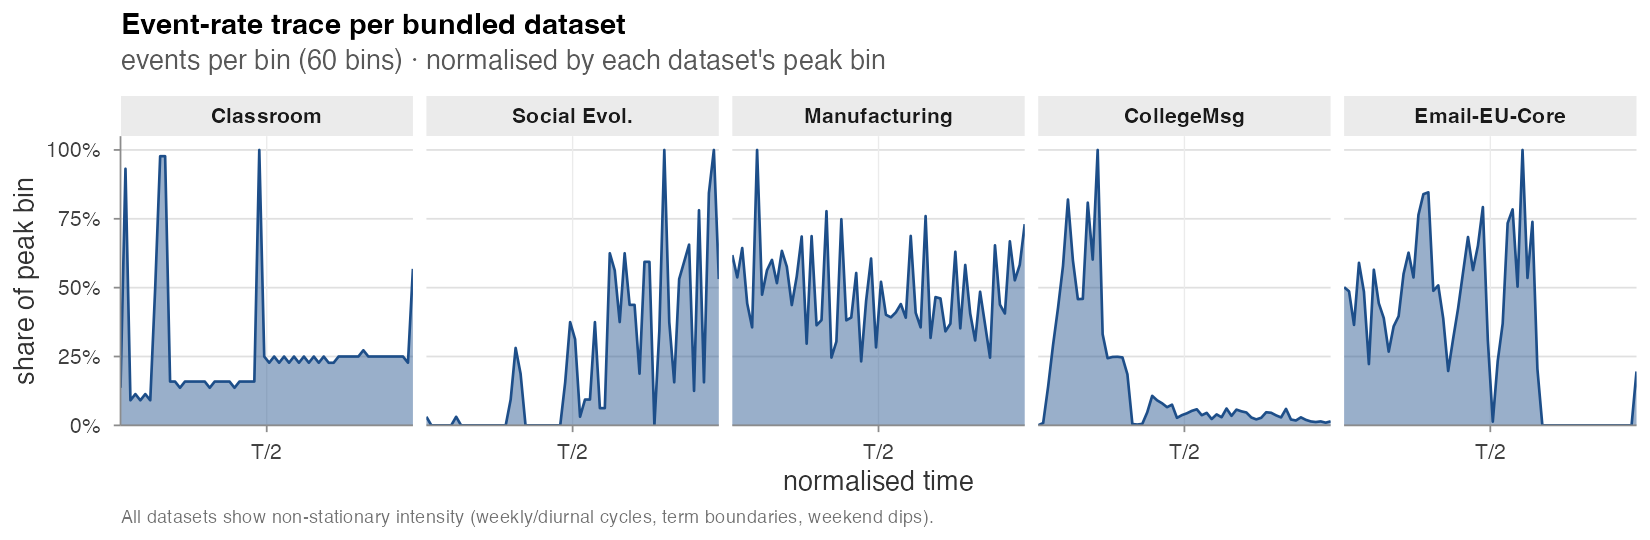
\includegraphics[width=0.8\linewidth]{figs/datasets-rate.png}
\caption{Event-rate profiles of the bundled event streams.}
\label{fig:datasets-rate}
\end{figure}

\begin{figure}[t]
\centering
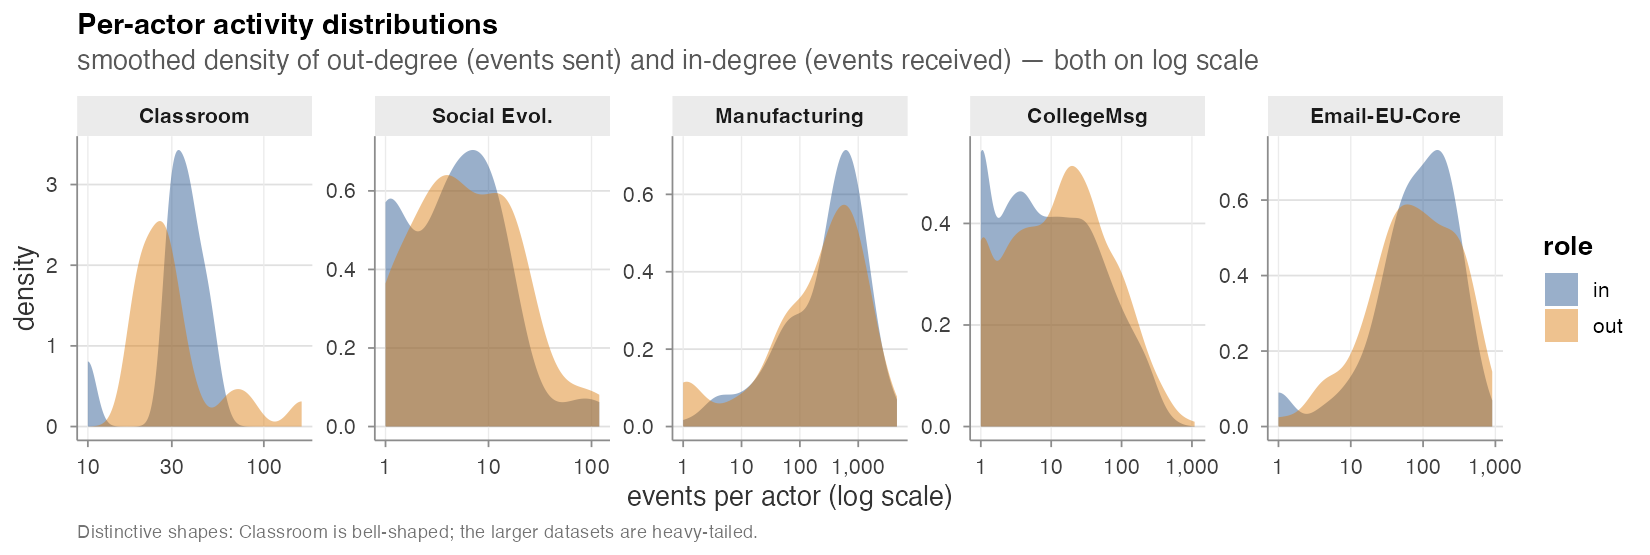
\includegraphics[width=0.8\linewidth]{figs/datasets-degrees.png}
\caption{Degree distributions across the bundled event streams.}
\label{fig:datasets-degrees}
\end{figure}

\begin{table}[t]
\centering
\caption{The nine bundled data objects. Event counts span 439 to 82{,}927
(\(\sim\)2 orders of magnitude). ``unix'' marks the four event streams that
carry \code{attr(., "unix\_origin")}.}
\label{tab:datasets}
\begin{tabular}{llrl}
\hline
Object & Kind & Rows & Source \\
\hline
\code{social\_evolution\_calls}      & event stream     & 439     & Madan et al.\ (2011), \emph{goldfish} \\
\code{classroom\_events}             & event stream     & 691     & McFarland (2001), \emph{networkDynamic} \\
\code{social\_evolution\_friendship} & event stream     & 766     & Madan et al.\ (2011), \emph{goldfish} \\
\code{email\_eu\_core}               & event stream     & 12{,}216 & Paranjape et al.\ (2017), SNAP \\
\code{college\_msg}                  & event stream     & 59{,}835 & Panzarasa et al.\ (2009), SNAP \\
\code{radoslaw\_email}               & event stream     & 82{,}927 & Michalski et al.\ (2014), Network Repository \\
\code{classroom\_actors}            & actor attributes & 20      & McFarland (2001) \\
\code{social\_evolution\_actors}     & actor attributes & 84      & Madan et al.\ (2011) \\
\code{dist\_matrix}                  & distance matrix  & 56\(\times\)56 & US Census TIGER/Line \\
\hline
\end{tabular}
\end{table}

\subsection{A worked end-to-end example}
\label{sec:software-example}

The following session takes \code{classroom\_events} --- 691 timestamped
directed interactions among 20 students \citep{McFarland2001} --- through the
full loop: sample non-events, fit a linear conditional logit, fit a smooth
counterpart, and check the fit.

\begin{verbatim}
library(amore)
data(classroom_events)

## 1. Sample one matched control per event from the full actor pool.
cc <- sample_non_events(classroom_events,
                        n_controls = 1, scope = "all", mode = "one",
                        seed = 11)

## 2. Compute endogenous statistics for cases and controls, reading the
##    true history but never letting controls update it.
feats <- compute_endogenous_features(
  cc,
  stats       = c("reciprocity_count", "transitivity_count"),
  history_log = classroom_events)

## 3a. Linear conditional logit (case-1-control => no-intercept binomial GLM).
fit <- rem(event ~ reciprocity_count + transitivity_count,
           data = feats, method = "clogit", stratum = "stratum")
coef(fit); summary(fit)

## 3b. The same data, widened, with a non-linear reciprocity effect.
w    <- widen_case_control(feats)
fitg <- rem(~ nl(reciprocity_count) + transitivity_count,
            data = w, method = "gam")
plot(fitg)                      # the fitted smooth panel

## 4. Goodness of fit of the linear specification.
m <- c(reciprocity_count = "linear", transitivity_count = "linear")
gof_univariate(classroom_events, m, "reciprocity_count", seed = 11)
gof_global(classroom_events, m, seed = 11)

## 5. Martingale residuals for diagnostic plotting.
res <- martingale_residuals(classroom_events, m, seed = 11)
plot(res$time, res$residual); abline(h = 0)
\end{verbatim}

Steps 3a and 3b illustrate the division of labour between backends: the
\code{clogit} fit gives interpretable linear coefficients on the matched
case-control strata, while the \code{gam} fit relaxes a chosen term to a smooth
on the case-1-control difference design. Steps 4 and 5 exercise the
goodness-of-fit family on the linear specification ---
Figure~\ref{fig:gof-process} shows the univariate cumulative residual process,
which starts and ends near zero under correct specification. The neural backend
is reachable from exactly the same upstream output by switching to
\code{method = "nn"} (Section~\ref{sec:validation}).

\begin{figure}[t]
\centering
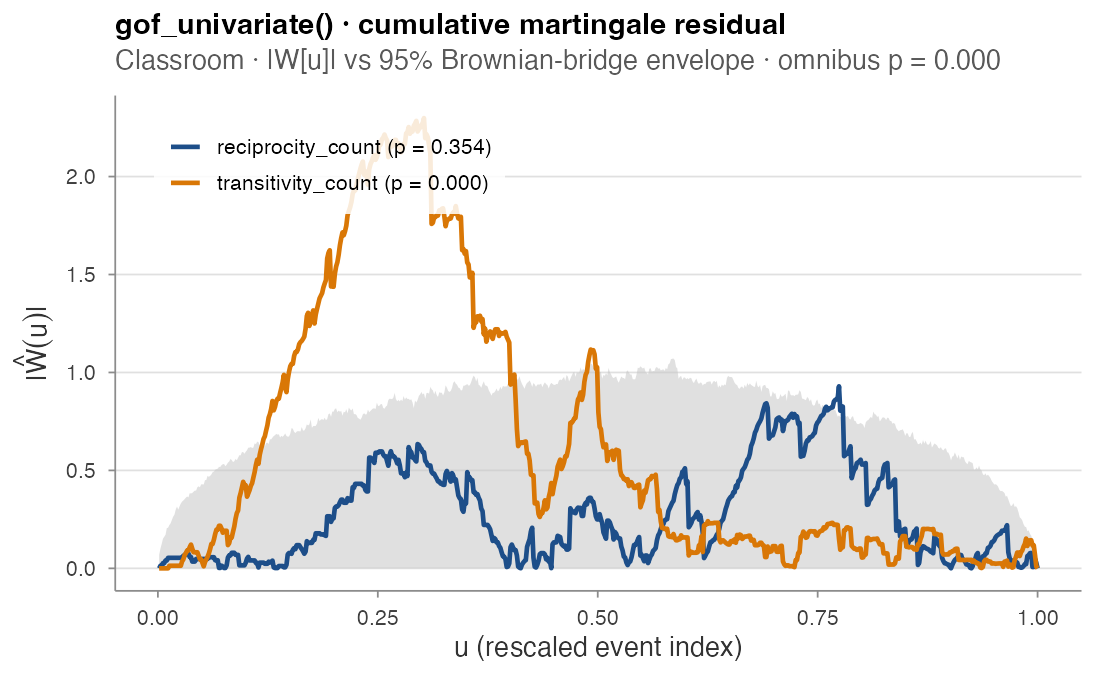
\includegraphics[width=0.7\linewidth]{figs/est-gof-process.png}
\caption{Univariate cumulative martingale-residual process for the
\code{reciprocity\_count} term on \code{classroom\_events}; under correct
specification the normalised process starts and ends near zero
\citep{boschi2025gof}.}
\label{fig:gof-process}
\end{figure}
